\documentclass[11pt]{article}
\usepackage[margin=1in]{geometry}
\usepackage[T1]{fontenc}
\usepackage{lmodern,microtype}
\usepackage{amsmath,amssymb,booktabs,array,graphicx}
\usepackage{caption,placeins}
\usepackage[numbers,sort&compress]{natbib}
\usepackage{url}
\usepackage[hidelinks]{hyperref}
\captionsetup{font=small,labelfont=bf}
\setlength{\emergencystretch}{2em}
\renewcommand{\topfraction}{0.9}
\renewcommand{\textfraction}{0.05}
\renewcommand{\floatpagefraction}{0.8}
\title{Reconstructing river dissolved organic carbon at unmonitored stations through environmental prediction and observation-aware residual transfer}
\author{Zhaochen Yang\\[2pt]\small Working manuscript --- October 2026}
\date{}
\begin{document}
\maketitle

\begin{abstract}
Sparse dissolved organic carbon (DOC) monitoring leaves many river stations without chemical observations needed to characterize aquatic carbon dynamics. Environmental learning provides a strong prediction reference, but transferring residual dynamics to an unmonitored station requires training under the same absence of local observations. We develop an environmental--temporal residual framework that combines station-hidden tree predictions, an ecological encoder, observation-aware recurrent memory and daily hydrological descriptors. Station-blocked cross-fitting supplies prediction errors for the recurrent branch; local DOC, pH and conductivity are absent in the principal new-station task. Five-seed geographical refits across five regions of a 357-station Mississippi cohort reduce equal-region MAE from 2.360 to 2.282~mg/L relative to the preceding complete model, a 3.31\% improvement with a paired station-bootstrap interval of 0.72--5.98\%. Deployment in an independently selected basin with 130 stations reduces zero-observation MAE from 0.984 to 0.915~mg/L, an improvement of 7.02\% [4.04--9.53\%]. A strong matched tree model achieves 0.841~mg/L there, while the residual model has lower station-equal error. Five designated observations reduce the upgraded model's external fixed-query MAE by 19.5\%. Source-calibrated intervals reach 84.9\% external coverage, illustrating the need to assess width and coverage together. The framework connects environmental prediction with transferable temporal correction and provides an explicit test of reconstruction without local chemistry. Further work will strengthen concentration-dependent residual transfer, high-DOC event reconstruction and basin-specific hydrological representation.
\end{abstract}
\paragraph{Keywords:} dissolved organic carbon; unmonitored rivers; ecological information; temporal memory; residual learning; geographical transfer

\section{Introduction}
River dissolved organic carbon links terrestrial carbon sources with downstream aquatic environments. Its concentration reflects catchment characteristics, hydrological conditions and biogeochemical processing, and varies substantially among regions \citep{yang2017}. Reconstructing missing DOC records supports comparisons among catchments and analysis of long-term aquatic carbon dynamics. Environmental and satellite-assisted learning already demonstrate the value of recovering river carbon patterns where direct measurements are incomplete \citep{tian2025}.

Monitoring remains uneven in both time and space. Water chemistry is sampled less continuously than meteorology or discharge, and available records differ among stations \citep{sterle2024}. A prolonged interruption at a monitored station can still leave useful local history. An unmonitored station has no such chemical reference. These are distinct reconstruction problems: improving predictions with nearby dates does not by itself establish transfer to a site without DOC observations.

Existing approaches provide complementary information. Interpolation and seasonal summaries exploit a station's observed history. Stream-network geostatistics represent flow connectivity and hydrological distance \citep{verhoef2006}. Random forests and extremely randomized trees capture nonlinear environmental relationships and can use explicit historical lags and neighboring-observation summaries \citep{breiman2001,geurts2006}. Recurrent graph models combine temporal and relational representations for missing-data reconstruction \citep{cini2022}; observation-aware recurrence can additionally use masks and elapsed time to represent irregular monitoring \citep{che2018}. Strong engineered-feature models therefore form a substantive comparison for a neural extension.

The transfer problem concerns how these information sources are learned and combined. A tree predictor can explain much of the environmental DOC signal, leaving residual variation for a temporal model. However, ordinary training rows may contain their station's chemical history even when the eventual target station has none. A residual learner trained on fitted tree errors faces a second mismatch: those errors can be much smaller than the errors at withheld stations. Both mismatches motivate training the correction on station-withheld prediction errors and station-hidden input histories.

We develop an integrated environmental--temporal residual model for DOC reconstruction without local chemistry. Environmental prediction supplies a reference, and an ecological encoder with observation-aware recurrent memory learns its remaining error under whole-station withholding. Source monitoring context and daily hydrology remain available. A small number of later-provided local observations can adjust the output through a separate station correction.

Our contributions are threefold. First, we align residual learning with the unmonitored-station information condition by jointly withholding station labels and their derived input histories. Second, we integrate environmental prediction, ecological encoding and hydrological temporal memory in a portable predictor for new station identities and calendars. Third, matched geographical refits and an independent basin evaluation identify the gain over the preceding complete model, the strength of explicit-feature trees and the added value of sparse local observations. The experiments thus connect the proposed method to the practical monitoring problem and indicate where its next improvements should concentrate.

\section{Materials and methods}
\subsection{Data and the unmonitored-station task}
The development cohort contains 357 Mississippi River stations, 324 directed river edges and 654 calendar months from April 1972 to September 2026. Only 22,571 of 233,478 station-month positions contain observed DOC (9.67\%). DOC concentration is in mg/L. Inputs include water temperature, discharge, their availability, calendar season, coordinates and ecological descriptors.

In the principal task, the receiving station has no DOC, pH or conductivity input. We hide its entire chemical history and the values, observation ages, masks and support features derived from that history. Source-station observations remain legitimate monitoring context. The resulting task represents reconstruction without a local chemical reference. Predictions are scored only where withheld DOC truth exists.

Eight bounded daily hydrological descriptors supplement the monthly inputs: three value descriptors and five coverage/availability descriptors constructed on the same discharge footprint. Current and previous months define retrospective monthly reconstruction; the task does not assume that a month's complete hydrology is known at its beginning. Twelve-month recurrent windows never include a future month.

\subsection{Environmental prediction and station-blocked residuals}
The environmental reference is an ExtraTrees predictor using 39 context features plus the eight daily descriptors. Four 300-tree configurations vary minimum leaf size (four, two or one) and all-feature versus square-root feature selection. Validation MAE selects the configuration. The ordinary daily-tree comparator fits rows with their original visible source history. The stronger station-hidden comparator fits each source row using its whole station fold's hidden-chemistry view. Both receive the same available inputs at the new station.

Five station folds generate out-of-fold (OOF) predictions. To predict a held station, a forest uses the other stations' labels and input context. For the station-hidden reference, inner station folds also hide local history in those fitting rows. This yields nested station-blocked errors with a train--deployment input condition matched to missing local chemistry.

Let $C^{\mathrm{OOF}}_{it}$ denote the withheld-station environmental prediction. The recurrent branch learns the native concentration residual
\[
 r^{\mathrm{OOF}}_{it}=y_{it}-C^{\mathrm{OOF}}_{it}.
\]
Validation and test use the environmental reference fitted to the full permitted training role. OOF predictions enter residual training; fitted training errors are not substituted for them.

\subsection{Ecological and observation-aware temporal correction}
The neural branch retains the ecological encoder and node self transformation of the existing graph model, with hidden width 64 and ecological embedding width 32. Its selected implementation uses empty neural edges. Explicit source-context features remain available, but this branch does not claim additional learned river-message propagation.

An observation-aware GRU encodes the previous twelve months. Its inputs describe monthly hydroclimate, season, ecological state, visible observation support and elapsed observation time. At an unmonitored station, local target-value and local-support channels remain zero; hydrological history, season and source context still inform the state. Daily hydrology, source-normalized ecology and predicted concentration additionally enter the existing residual readout through additive features and fixed interactions.

For a full-fit environmental prediction $C_{it}$, the native residual expert is
\[
 P^{\mathrm{native}}_{it}=\max\{0,C_{it}+s\,d_\theta(h_{it},x_{it})\},
\]
where $s\in\{0,0.25,0.5,1\}$ is selected on validation MAE. A zero-initialized head starts at the environmental reference. Absolute-error training retains a weight of two for training-derived Q90 DOC cells. No upper concentration clipping is applied.

The fixed recipe first fits a fresh observation-aware backbone (20-epoch cap), then the preceding daily native residual (120-epoch cap), and finally the station-hidden candidate (30 extra epochs). Early-stopping patience is five. The candidate inherits fitted ecological and recurrent states while initializing its new residual head at zero. The procedure comparison includes this additional optimization budget.

Source OOF errors can also supply ecological-neighbor residual profiles. Validation selects their blending weight, including an exact zero-memory option. The selected complete procedure is fixed before geographical and external evaluation; native-only is retained as an ablation. Dynamic and target statistics use source training cells. Historical coordinate/ecology preprocessing retains the known development-cohort convention and is saved for deployment; scales are not re-estimated on a new target cohort.

\begin{figure}[!htbp]\centering
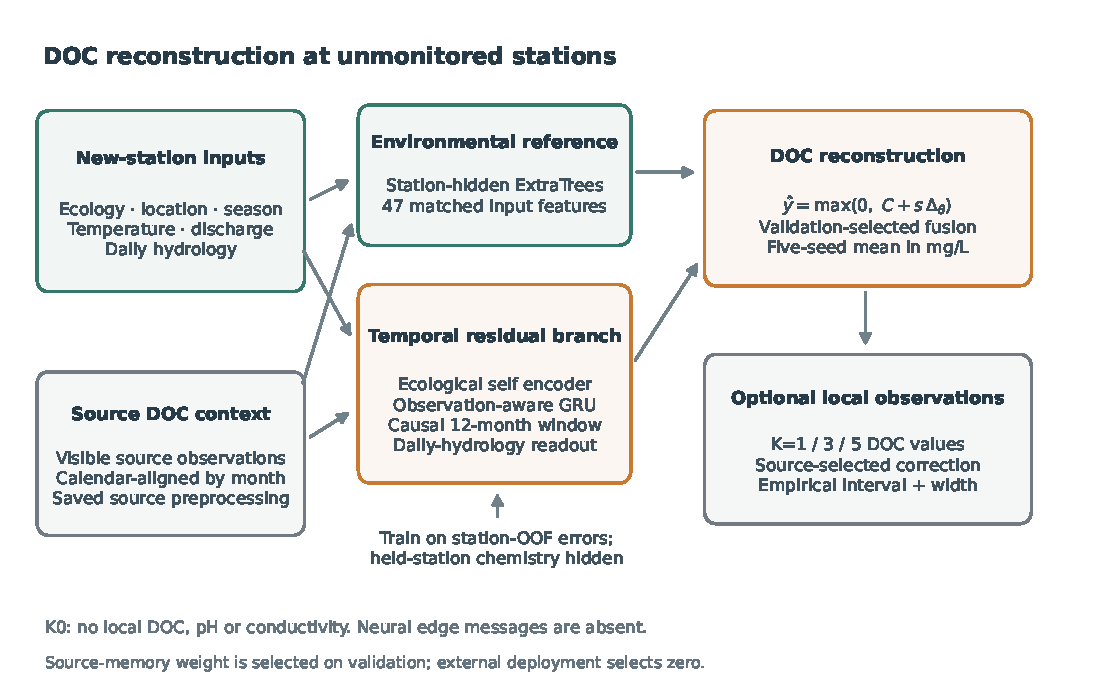
\includegraphics[width=\linewidth]{figures/doc_deployment_architecture_v1.pdf}
\caption{\textbf{Environmental prediction and observation-aware residual transfer.} Station-hidden trees provide a concentration reference. The retained ecological/self encoder and recurrent memory learn its source OOF error using monthly context and daily hydrology. Validation selects the residual scale and optional source-memory fusion. K0 uses no new-station chemistry. A separate output correction accepts designated DOC supports. The external deployment selects zero ecological-memory weight in every seed; empty neural edges are retained.}
\label{fig:architecture}
\end{figure}

\subsection{Geographical refits and independent deployment}
We rotate five sufficiently populated HUC4 regions: 1013, 1019, 0708, 1030 and 1101. Each is withheld for test, the next region cyclically supplies validation, and the remainder trains. Every role assignment is fitted afresh with seeds 42--46. Main K0 scores all 7,262 valid test DOC cells at 104 stations, including sparse stations. Region metrics first average seed errors and then weight the five regions equally. These are retrospective geographical tests within ST357.

The independent external case, HUC02040104, is selected from previously ordered candidates using DOC availability and common-input construction. It contains 130 stations disjoint from ST357, 520 calendar months and 6,514 DOC observations. Temperature is available at 96.5\% of DOC cells and discharge at 34.1\%. Prediction outcomes do not select the case.

For deployment, 303 ST stations with 20,288 DOC cells train the model; 54 fixed source-validation stations provide 2,283 cells for selection. Historical internal test stations legitimately become source observations for this independent deployment. Five fresh source fits preserve the fixed recipe. All procedures use an arithmetic mean of native-mg/L predictions. Point products and source-validation policies are saved before external DOC is opened for scoring. No external DOC calibrates K0.

Portable prediction uses saved preprocessing, source observations and source error experience. It accepts arbitrary new station identities and consecutive calendars, without ST357 node indices. Source context is matched by calendar month. Named source-to-external river links are absent in this case, so directional context is zero; the no-message neural recipe remains applicable.

\subsection{Temporal compatibility refits}
We additionally refit the station-hidden native recipe on two existing monitored-station time tasks: unobserved periods and periods with designated observation assistance. Each uses seeds 42--44, its original train/validation/test/context cells and fresh source fitting. Past local chemistry remains available where allowed by the temporal role. The ecological-neighbor module is omitted because training and validation station identities overlap. The existing validation-selected fusion family combines environmental and native predictions, including a log-affine concentration adjustment. Results average individual-seed errors within each time split and provide a retrospective compatibility assessment distinct from the portable new-station deployment.

\subsection{Sparse observations and uncertainty}
Five dates per eligible station are reserved in the order first, middle, last, first quartile and third quartile. Nested prefixes define $K=0,1,3,5$. All five candidates are excluded from the curve query at every K, leaving 5,864 external query cells. This curve population differs from the all-observation primary K0 population.

For a support set $\mathcal S_i$, adaptation adds a shrunken mean log residual:
\[
 \widehat y_{it}^{(K)}
 =\max\!\left\{0,\exp\!\left[\log(1+P_{it})
 +\frac{\alpha_K}{K}\sum_{s\in\mathcal S_i}
       \bigl(\log(1+y_{is})-\log(1+P_{is})\bigr)\right]-1\right\}.
\]
K0 returns the original prediction. Source-validation ensemble query MAE selects $\alpha_K$ from $\{0,0.25,0.5,0.75,1\}$; ties favor a smaller value. Only designated external supports enter adaptation. Supports may follow query dates, so the correction is retrospective.

Source validation supplies a finite-rank 90\% quantile of absolute log1p prediction errors. Intervals transform the prediction plus/minus that constant log half-width back to nonnegative concentration. Matching adapted source-validation queries calibrate each K curve. Because validation also selects the model, these are empirical intervals. We report coverage jointly with native interval width and high-DOC coverage.

\subsection{Evaluation}
Main comparisons retain the preceding complete model, ordinary matched daily trees, strong station-hidden trees, the native ablation and the fixed complete upgrade. MAE is primary; RMSE, bias, station-equal MAE and training-derived Q90 diagnostics complement it. Station-equal and cell-weighted errors answer different weighting questions and are not interchangeable. Q90 groups with fewer than 20 unique cells are marked unstable.

Paired 95\% intervals use 5,000 station-bootstrap draws, carrying a station's months together. Geographical analysis preserves region weighting; the external analysis describes station sampling within one independent basin. Repeated seeds do not add ecological samples. Source-defined ecological novelty, nearest-source distance and hydro availability provide descriptive strata. Structured evaluation follows the intended reconstruction setting \citep{roberts2017}. All temporal development results remain distinct from the new geographical and external evaluations.

\FloatBarrier
\section{Results}
\subsection{The upgrade improves reconstruction across withheld regions}
The fixed complete upgrade achieves equal-region K0 MAE 2.282~mg/L, versus 2.360 for the preceding complete model (Table~\ref{tab:geo}). The reduction is 3.31\%, with a paired station-bootstrap interval of 0.72--5.98\%; three of five regions improve. Relative to strong station-hidden trees (2.345~mg/L), the reduction is 2.67\% [$-0.04$,5.15\%], with positive directions in all five regions. Its estimated gain is consistent in direction but not established by the overall interval against that stronger comparator.

\begin{table}[htbp]\centering\small
\caption{Five-seed geographical reconstruction, with equal region weighting. Errors are in mg/L. Q90 thresholds come from each task's source training role.}
\label{tab:geo}
\begin{tabular}{lrrr}\toprule
Procedure & MAE & Station-equal MAE & Q90 MAE\\\midrule
Preceding complete model &2.360&2.557&10.632\\
Ordinary matched daily trees &2.441&2.606&10.474\\
Strong station-hidden trees &2.345&2.548&10.520\\
Native residual ablation &2.266&2.485&10.494\\
Fixed complete upgrade &2.282&2.505&10.520\\\bottomrule
\end{tabular}
\end{table}

The native residual ablation scores 2.266~mg/L, slightly below the complete upgrade. The source-selected memory fusion therefore adds no overall geographical gain. The Q90 improvement over the preceding complete model is 1.06\% with an interval crossing zero. Two regional tail groups contain fewer than 20 cells. High-concentration reconstruction remains a distinct challenge.

\begin{figure}[!htbp]\centering
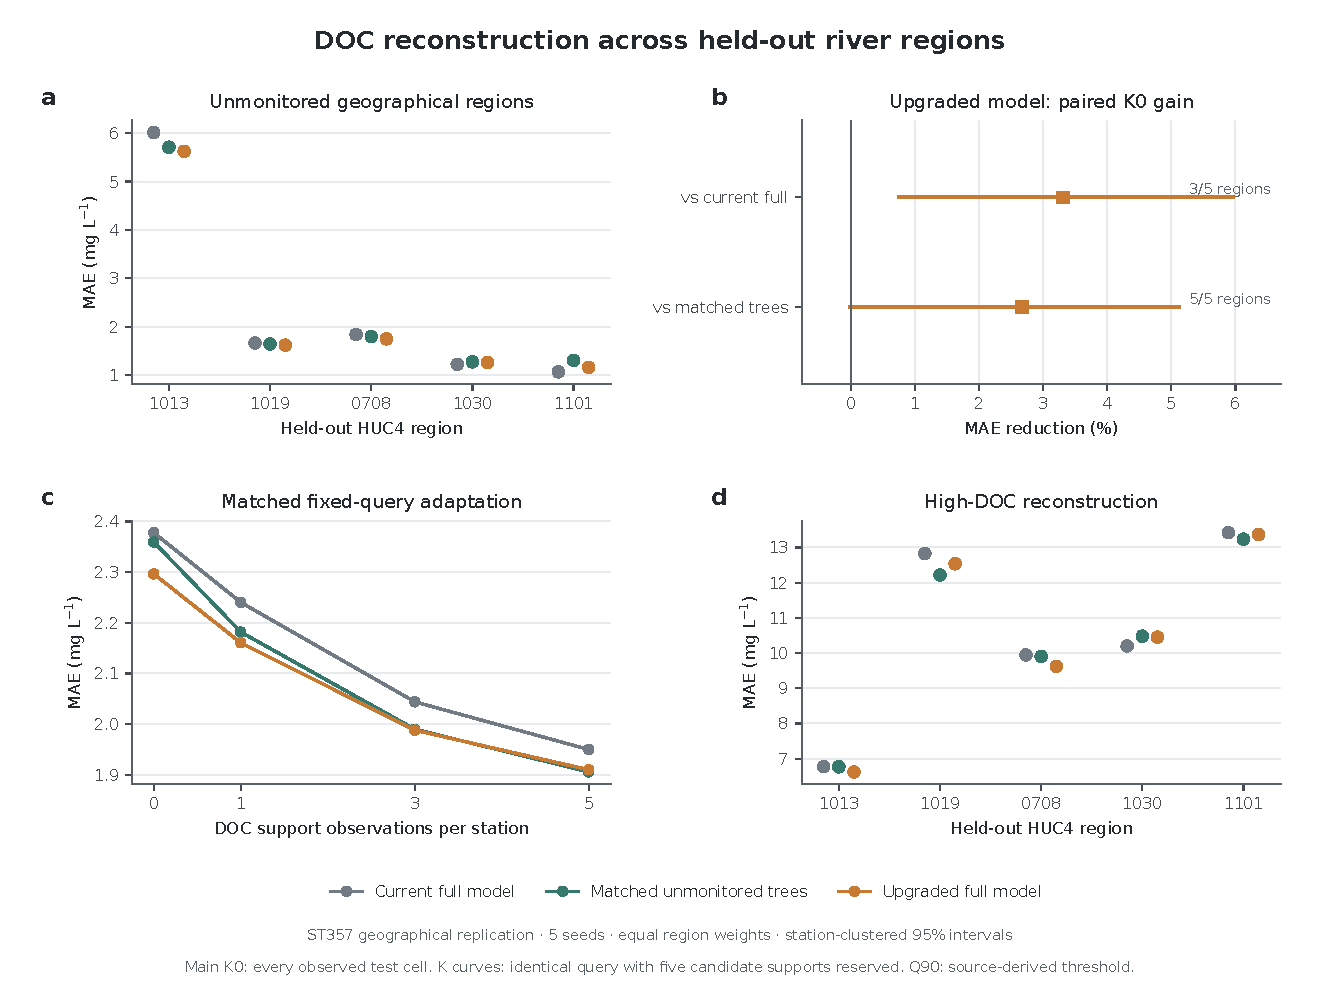
\includegraphics[width=\linewidth]{figures/doc_geographical_confirmation_v1.pdf}
\caption{\textbf{DOC reconstruction across five withheld regions.} Matched five-seed refits preserve test regions and query cells. Region-level variation, paired station intervals, fixed-query support curves and tail diagnostics describe the complete upgrade and its fixed comparators. This experiment is ST357 geographical replication, rather than the independent basin deployment.}
\label{fig:geo}
\end{figure}

\subsection{Zero-observation reconstruction transfers to an independent basin}
The upgraded ensemble reduces external K0 MAE from 0.984 to 0.915~mg/L relative to the preceding complete model: 7.02\% [4.04,9.53\%]. Strong station-hidden trees score 0.841~mg/L; the upgrade's relative gain against them is $-8.82$\% [$-19.43$,3.47\%] (Figure~\ref{fig:external}). The model therefore improves its preceding complete prediction procedure beyond ST357, while explicit-feature trees remain a strong competitor.

The station-equal summary reverses this point-estimate ordering: upgraded MAE is 0.841~mg/L, versus 0.905 for strong trees. Stations have unequal observation counts, so the two summaries emphasize different station records. This result motivates attention to monitoring effort without changing the principal cell-weighted endpoint.

All five source deployment fits select ecological-memory weight zero on source validation. Consequently the complete and native-only predictions coincide in this deployment. The observed improvement does not establish an extra retrieval-memory contribution.

\begin{figure}[!htbp]\centering
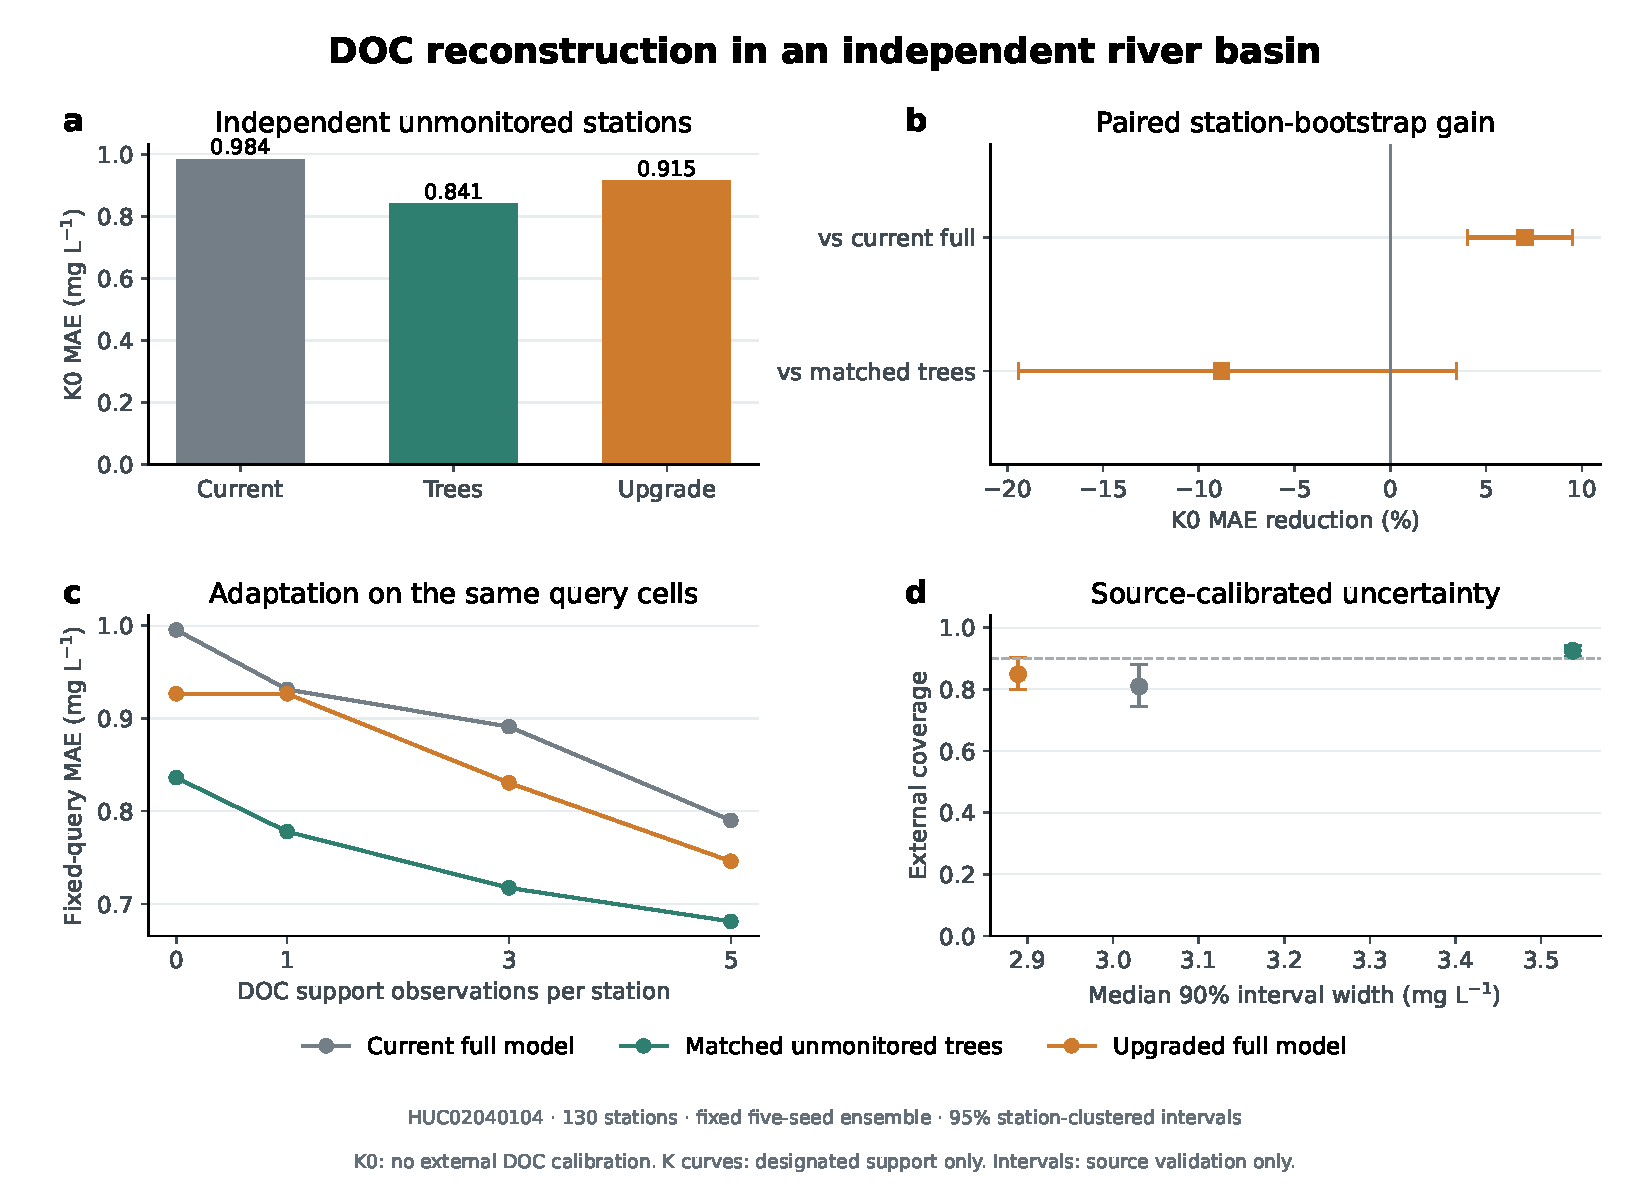
\includegraphics[width=\linewidth]{figures/doc_external_replication_v1.pdf}
\caption{\textbf{Independent basin reconstruction without local chemistry.} \textbf{a,} K0 MAE on 6,514 cells at 130 stations. \textbf{b,} Relative gain with paired station-bootstrap intervals. \textbf{c,} Adaptation on the same 5,864 query cells at every K. \textbf{d,} Source-validation empirical interval coverage and median width. Points use a fixed five-seed mean; no external DOC selects the K0 predictor, adaptation strength or interval scale.}
\label{fig:external}
\end{figure}

\subsection{Environmental support reveals different transfer regimes}
Figure~\ref{fig:conditions} compares the same models across source-defined environmental strata. In the geographical experiment, the upgrade improves on the preceding model across hydrological availability groups; ecological and nearest-source distance groups have different regional populations. These summaries describe the usable regions within each stratum.

In the independent basin, one available hydro channel gives upgraded MAE 0.818~mg/L versus 0.849 for strong trees. With both channels available, the upgraded error rises to 1.114~mg/L while the tree error remains 0.831~mg/L. The ecological high-novelty group contains 12 stations, and 128 of the 130 external stations lie in the high nearest-source-distance group. Such uneven source-to-target coverage provides a concrete setting for further residual-transfer research.

\begin{figure}[!htbp]\centering
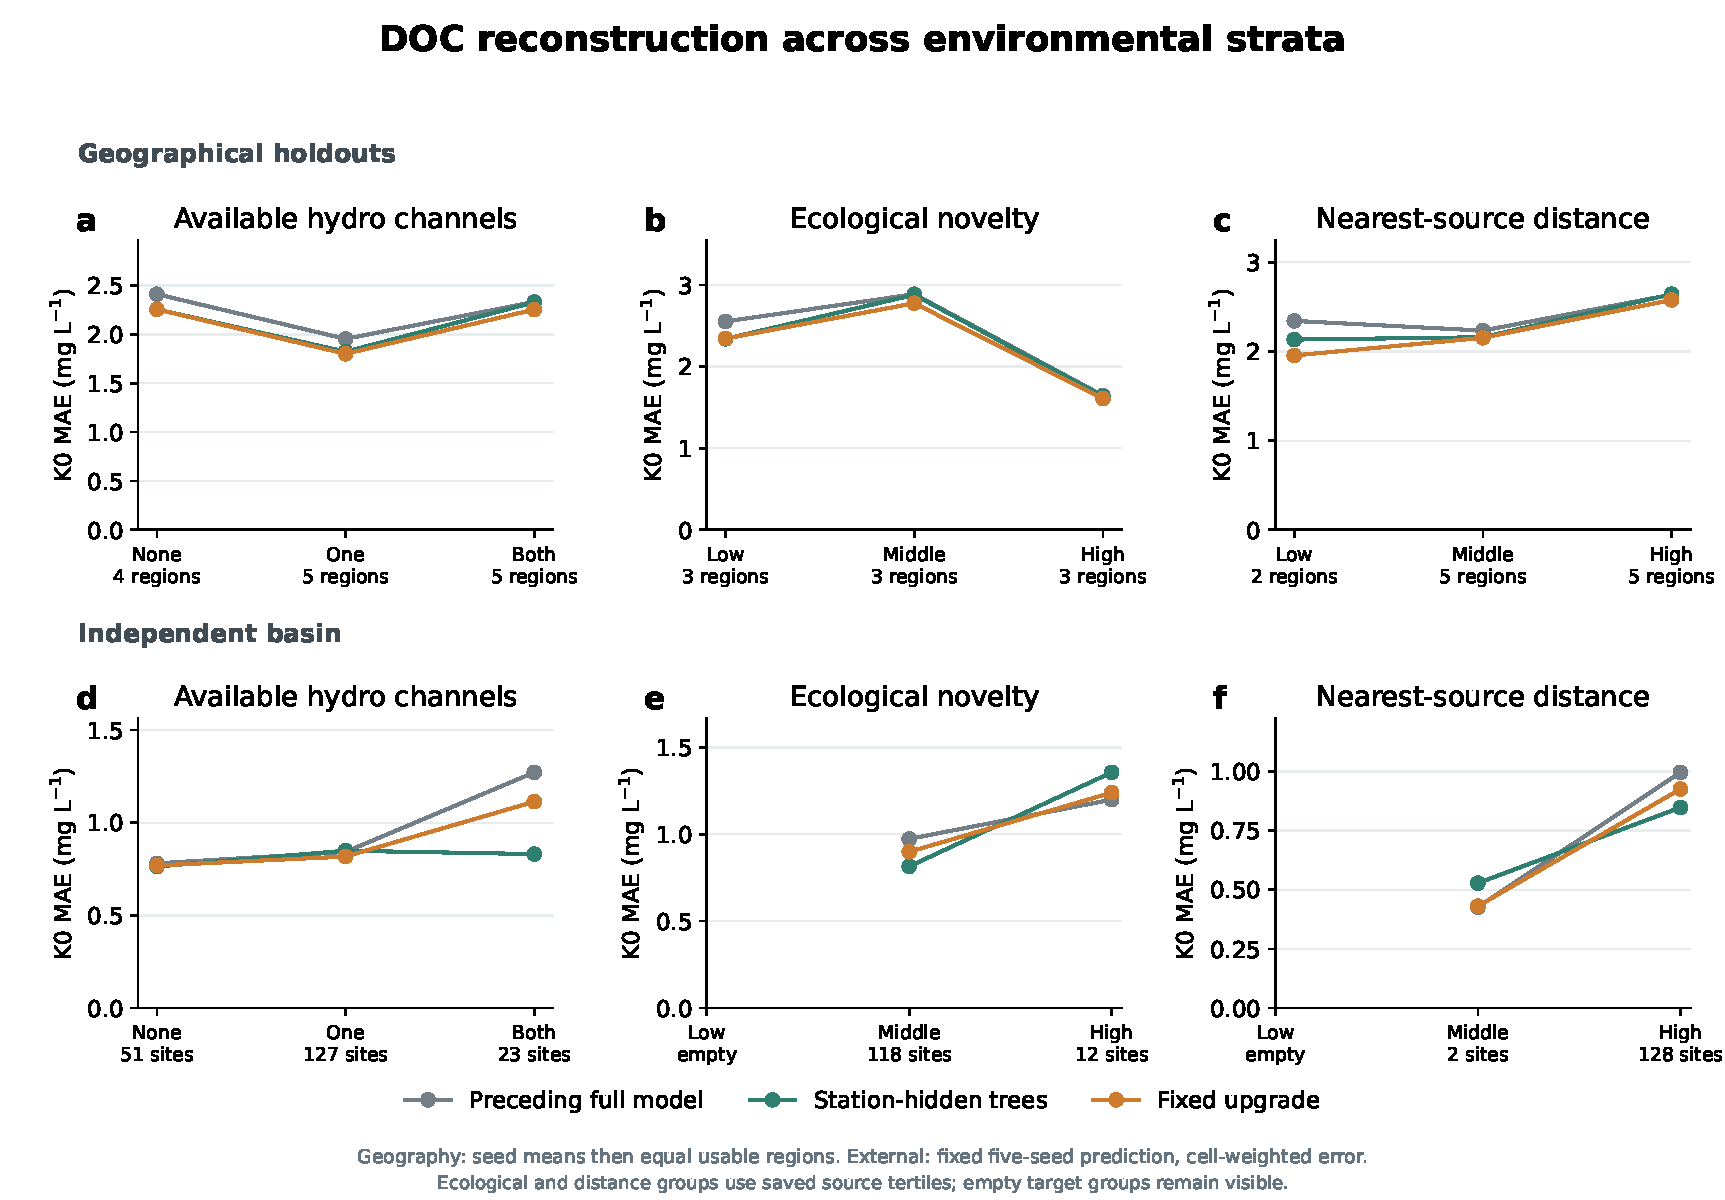
\includegraphics[width=\linewidth]{figures/doc_transfer_conditions_v1.pdf}
\caption{\textbf{Reconstruction across environmental and hydrological conditions.} The top row reports seed means averaged over usable geographical regions; the bottom row reports cell-weighted error for the external five-seed ensemble. Source-defined tertiles classify ecological novelty and nearest-source distance. Numbers identify contributing regions or unique stations. A station can occur in several hydro-availability groups across months. Empty external groups remain displayed.}
\label{fig:conditions}
\end{figure}

\subsection{A few local observations improve the reconstructed record}
On fixed external queries, upgraded MAE decreases from 0.927 at K0 to 0.831 at K3 and 0.746~mg/L at K5: a 19.5\% reduction. Its K1 output is unchanged because source validation selected zero correction strength. The preceding complete model reaches 0.790~mg/L at K5, while equally adapted strong trees reach 0.681~mg/L. Sparse observations help both model families, and their value is evaluated on an unchanged query population.

\subsection{Uncertainty and high DOC require separate evaluation}
Nominal 90\% source-calibrated intervals achieve 84.9\% external coverage [80.0,90.3\%], with median width 2.889~mg/L. Strong trees achieve 92.5\% [90.5,94.3\%] with median width 3.537~mg/L. The wider tree interval covers more external observations. Neither overall MAE nor interval coverage alone describes all operational performance.

The source-training Q90 threshold is 9.730~mg/L, identifying only 16 external cells at 11 stations. All procedures have zero recall and interval coverage for these cells. Upgraded Q90 MAE is 9.566~mg/L, versus 9.392 for strong trees. These sparse tail data describe missed high-DOC observations and are not a stable estimate of broad tail behavior.

\subsection{The updated procedure retains temporal reconstruction performance}
Fresh temporal refits produce upgraded full-fusion MAE of 0.786~mg/L in unobserved periods and 0.798~mg/L in observation-assisted periods (Figure~\ref{fig:time}). Corresponding strong station-hidden trees score 0.897 and 0.936~mg/L: reductions of 12.41\% [8.60,15.84\%] and 14.81\% [11.79,17.55\%]. Against current full temporal fusion, reductions are 13.19\% [3.91,20.69\%] and 6.55\% [$-2.32$,13.45\%]. All three seeds improve in each current-fusion contrast, while the assisted-period interval remains uncertain.

The upgraded native residual alone reduces tree error by only 0.24\% and 0.29\%, with both intervals crossing zero. All six complete refits select log-affine validation fusion; seed42 selects zero native residual scale. The full-procedure improvement thus includes concentration/bias calibration, and additional neural-memory value requires a calibrated tree-only comparison. These temporal results concern legitimate local-history tasks and separately fitted procedures. Their Q90 groups contain only 12 and seven cells.

\begin{figure}[!htbp]\centering
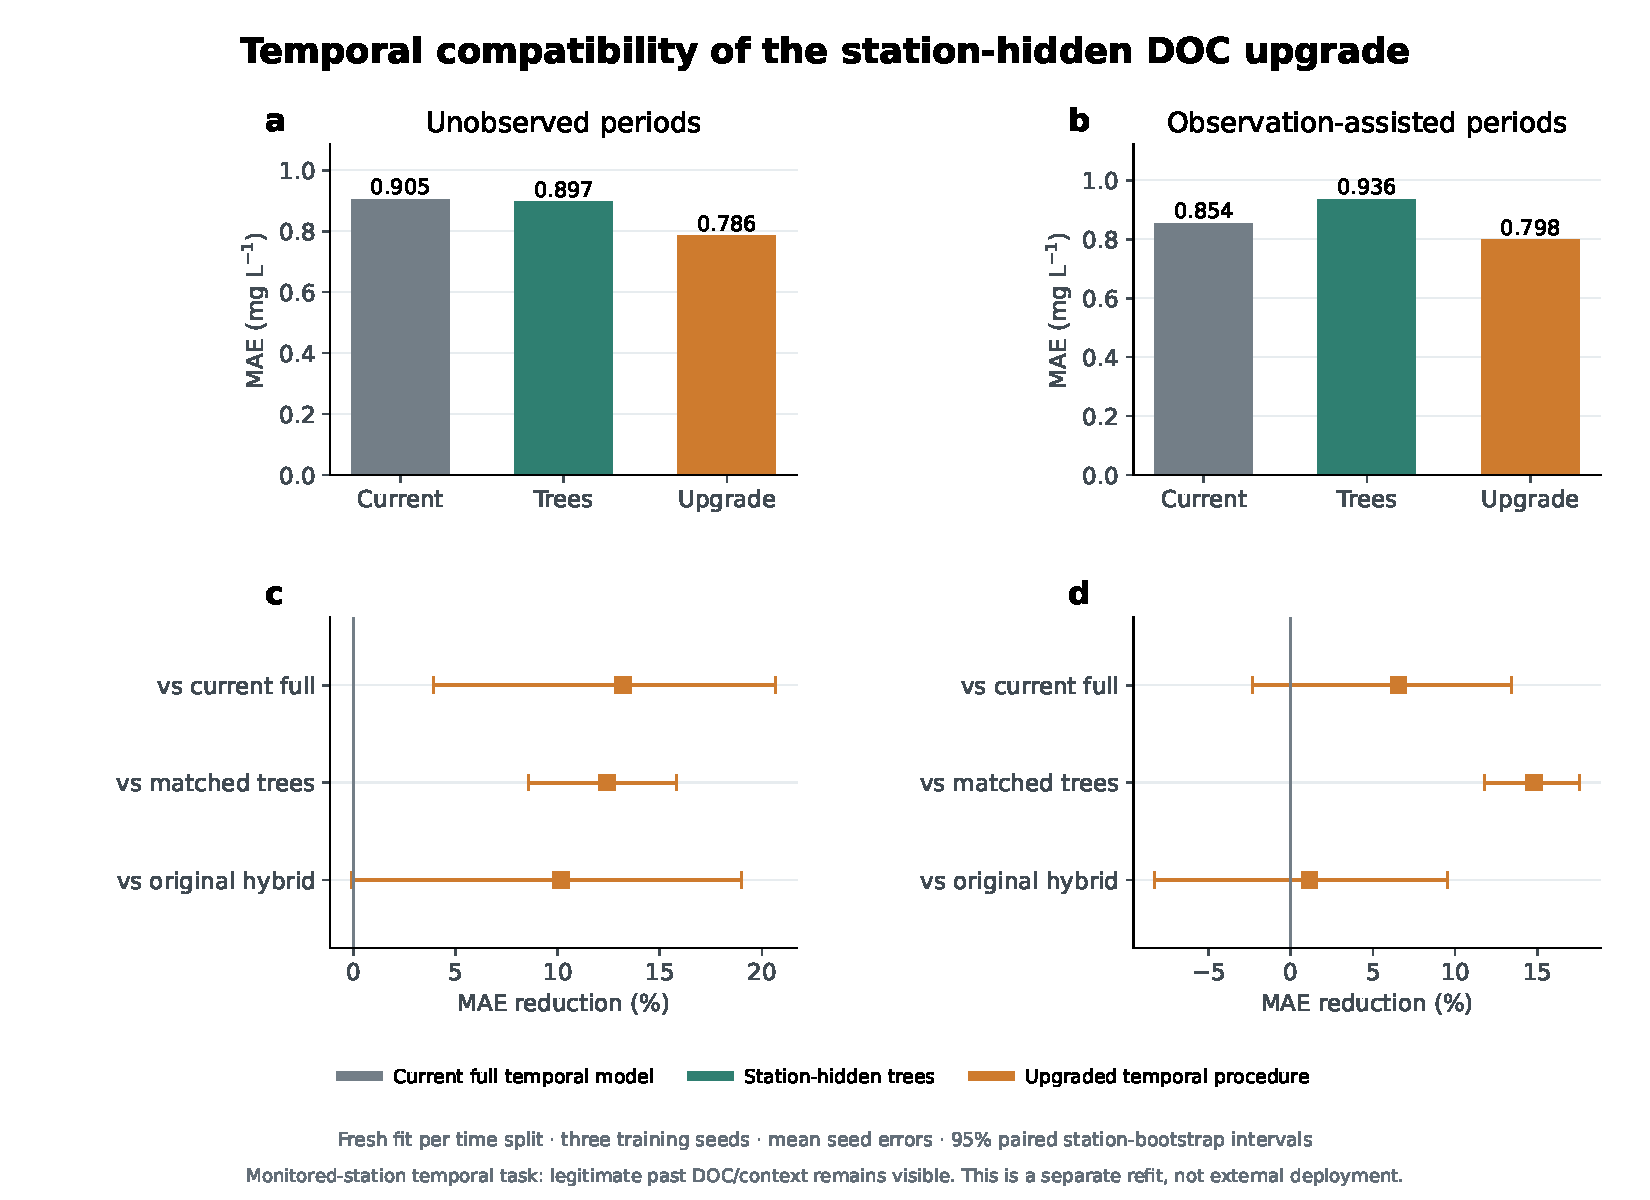
\includegraphics[width=\linewidth]{figures/doc_temporal_compatibility_v2.pdf}
\caption{\textbf{Temporal reconstruction after the station-hidden upgrade.} Fresh three-seed procedures use the original monitored-station temporal roles. The top panels show mean individual-seed errors; the bottom panels show paired station-bootstrap gains against current full fusion, strong station-hidden trees and the original twenty-epoch hybrid. Native-only gain and selected validation fusion are reported separately to distinguish complete-procedure performance from a neural contribution.}
\label{fig:time}
\end{figure}

\FloatBarrier
\section{Discussion}
\subsection{Matching residual learning to sparse monitoring}
The proposed division of prediction gives each component a concrete role. Environmental trees provide nonlinear background prediction; recurrent learning targets the error observed when a station is withheld. Hiding its input history as well as its fitting labels aligns this correction with the absence of local chemistry at deployment. This is the central method contribution, rather than a claim that graph depth or topology explains every observed gain.

Geographical and independent-basin results show improvement over the preceding complete model. The comparison against matched trees also identifies the remaining prediction challenge. Engineered ecological and hydrological features can be highly effective, and a neural correction can add bias when transferred to another concentration regime. External upgraded mean bias is $-0.434$~mg/L, versus $-0.034$ for strong trees. The largest descriptive gap occurs where both hydro channels are available. These strata identify environments for further investigation; they do not prove a mechanism.

\subsection{Transfer, monitoring effort and local information}
The different cell-weighted and station-equal external summaries demonstrate why station records must be considered explicitly. A source-only matched experiment tested equal-station residual loss with unchanged architecture, 30-epoch budget and within-station Q90 weight. It produced $-0.12$\% relative gain [$-0.65$,0.39\%] against the existing complete upgrade, improving only one of three development partitions. This simple change is not adopted. Monitoring-frequency differences remain useful descriptive evidence, while their remedy requires more than reweighting alone.

The external correction curve shows how a small number of local measurements can complement zero-observation transfer. Current supports adjust concentration reference without changing recurrent dynamics. This separates the contribution of new local evidence from the transferable prediction learned at source stations.

\subsection{Future research directions}
First, residual transfer should represent differences in concentration regime and hydrological observation support more directly. Source-only experiments can test concentration-scaled corrections and hydrological state representations before further geographical testing. Additional independently selected basins would determine whether the present external behavior is shared across catchment environments.

Second, event-sensitive reconstruction requires higher-frequency DOC paired with rainfall and flow, so that a model can learn peak magnitude and timing. The 16 external source-Q90 cells are insufficient for a detailed transport interpretation. Process states and reliable reach flow/source information could enrich river-message modeling beyond the currently selected no-message branch.

Third, local adaptation can move from a station-level output adjustment to observation-conditioned state updates. Comparing retrospective support with observations available before each prediction would connect reconstruction to ongoing monitoring.

Finally, uncertainty should track distribution shift while preserving useful interval width. The current external coverage--width comparison and earlier uncertainty-ranking diagnostics provide a starting point. Concentration and flow uncertainty would need joint propagation before using reconstructed monthly DOC for carbon-load assessment.

\section{Conclusion}
We developed a portable environmental--temporal residual framework for DOC reconstruction at stations without local chemistry. Station-blocked errors and station-hidden input histories align neural correction with the intended monitoring condition. The fixed procedure improves on the preceding complete model by 3.31\% across internal geographical holdouts and 7.02\% in an independently selected basin. Five local observations provide a further 19.5\% reduction on fixed external queries. Strong explicit-feature trees retain lower external cell-weighted error, highlighting concentration-dependent residual transfer and high-DOC dynamics as the next priorities. These findings link the method to a practical reconstruction need and define a direct route for its continued improvement.

\section*{Data, code and figure availability}
The source-only development, five-region confirmation, portable source fits and independent basin evaluation retain configurations, predictions, source snapshots and reproducible analyses in separate version directories. The current model exposes fitting, prediction, component prediction and saved-state restoration; the five-seed deployment bundle also contains source-selected support and interval policies. The geographical, external and temporal analyses use 5,000 paired station draws. All figures in this draft are code-generated from the implemented model and saved numerical evidence. The older manuscript and its historical experiments remain available. A persistent public data/code release identifier has not yet been assigned.

\begin{thebibliography}{99}
\bibitem{yang2017}Yang, Q., Zhang, X., Xu, X., and Asrar, G.~R. (2017). An analysis of terrestrial and aquatic environmental controls of riverine dissolved organic carbon in the conterminous United States. \emph{Water},9,383. \url{https://doi.org/10.3390/w9060383}.
\bibitem{tian2025}Tian, S., Sha, A., Luo, Y., et al. (2025). A novel framework for river organic carbon retrieval through satellite data and machine learning. \emph{ISPRS Journal of Photogrammetry and Remote Sensing},221,109--123. \url{https://doi.org/10.1016/j.isprsjprs.2025.01.028}.
\bibitem{sterle2024}Sterle, G., Perdrial, J., Kincaid, D.~W., et al. (2024). CAMELS-Chem: augmenting CAMELS with atmospheric and stream water chemistry data. \emph{Hydrology and Earth System Sciences},28,611--630. \url{https://doi.org/10.5194/hess-28-611-2024}.
\bibitem{verhoef2006}Ver Hoef, J.~M., Peterson, E., and Theobald, D. (2006). Spatial statistical models that use flow and stream distance. \emph{Environmental and Ecological Statistics},13,449--464. \url{https://doi.org/10.1007/s10651-006-0022-8}.
\bibitem{breiman2001}Breiman, L. (2001). Random forests. \emph{Machine Learning},45,5--32. \url{https://doi.org/10.1023/A:1010933404324}.
\bibitem{geurts2006}Geurts, P., Ernst, D., and Wehenkel, L. (2006). Extremely randomized trees. \emph{Machine Learning},63,3--42. \url{https://doi.org/10.1007/s10994-006-6226-1}.
\bibitem{cini2022}Cini, A., Marisca, I., and Alippi, C. (2022). Filling the G\_ap\_s: multivariate time series imputation by graph neural networks. \emph{ICLR}. \url{https://openreview.net/forum?id=kOu3-S3wJ7}.
\bibitem{che2018}Che, Z., Purushotham, S., Cho, K., Sontag, D., and Liu, Y. (2018). Recurrent neural networks for multivariate time series with missing values. \emph{Scientific Reports},8,6085. \url{https://doi.org/10.1038/s41598-018-24271-9}.
\bibitem{roberts2017}Roberts, D.~R., Bahn, V., Ciuti, S., et al. (2017). Cross-validation strategies for data with temporal, spatial, hierarchical, or phylogenetic structure. \emph{Ecography},40,913--929. \url{https://doi.org/10.1111/ecog.02881}.
\end{thebibliography}
\end{document}
